\documentclass[11pt]{article}
\renewcommand{\baselinestretch}{1.20} 
\usepackage[authoryear,round,longnamesfirst]{natbib}
\usepackage[utf8]{inputenc}
\usepackage[danish]{babel}
\usepackage{graphicx}
\usepackage{subfigure}
\usepackage{subcaption}
\usepackage{pdfpages}
\usepackage{caption}
\usepackage{geometry}
 \geometry{
 a4paper,
 total={170mm,237mm},
 left=20mm,
 top=30mm,
 }
\usepackage{fancyhdr}

\pagestyle{fancy}
\fancyhf{}
\rhead{Social hidden Messages 2018}
\lhead{Gruppe: B-125}
\chead{P2 - Rapport}
\rfoot{Page \thepage}

\usepackage{titlesec}

\setcounter{secnumdepth}{4}

\titleformat{\paragraph}
{\normalfont\normalsize\bfseries}{\theparagraph}{1em}{}
\titlespacing*{\paragraph}
{0pt}{3.25ex plus 1ex minus .2ex}{1.5ex plus .2ex}

\title{P2 - Hidden messages through the media \\ Gruppe: B-125}

\author{
    \\
    Udarbejdet af:\\
    \\
    Mikkel Steen Hansen\\
    Martin Boe\\
    Benjamin Jensen\\
    Daniel Jensen\\
    \\
    Vejleder:\\ 
    \\
    Rasmus Løvenstein Olsen\\
}
\date{\textbf{ 6. February 2018}}

\begin{document}

\begin{titlepage}
\clearpage
\maketitle
\thispagestyle{empty}

\end{titlepage}

\renewcommand{\baselinestretch}{0.8} 
\tableofcontents
\renewcommand{\baselinestretch}{1.20} 
\newpage

\section{Indledning}
Siden mennesket har kunne kommunikere med hinanden, har det også haft behov for at skjule en sandhed eller et budskab. \cite{PastCryptography} Dog har nogle af disse hemmeligheder også senere haft brug for enten at blive gemt, eller delt mellem enkelte individer. Problemet opstår her i, at en nedskreven hemmelighed har lettere ved at blive røbet, og at delingen af denne også kan komme til ikke tiltænkte individer.
Derfor har man altid arbejdet i at kunne kryptere, formatere, eller med andre ord skjule, beskeder til alle tænkelige former for brug, lige fra militante strategier, til deling af videns-studier. \cite{The_Invention_of_the_Internet} \\
Hertil er det dog vigtigt, at være klar over at kryptologi, som betyder "læren om det hemmelige", er et paraplyudtryk. Inden under dette hører blandt andre kryptografi, som nok er den mest kendte sikkerheds foranstaltning, og som er grundlaget for at skjule indeholdet af en besked. Et andet koncept, som hører under kryptologi er steganografi. Dette er anderledes i det, at steganografi handler om, at skjule eksistensen af en besked i stedet for indholdet.\cite{MeningOfCryptography} \quad \cite{MeningOfSteganografi}
I dag arbejdes der stadig hårdt på at udvikle nye metoder til at skjule meddelelser, faktisk med nutidens udbredelse af netværksbaseret løsninger, har behovet for disse metoder af datasikringer aldrig været større.\cite{Internetsikkerhed_forlav} Næsten alle i de industrialiseret lande er i dag online, på det ene eller det andet sociale medie, og selv små lande er igennem internettet eksponeret til resten af verdenen. Da kommunikation over internettet involverer flere elementer end blot de to endpoints, passer dette også godt ind i det overordnede semestertema, som er netværksbaseret databehandling.

Instagram er en kogebog i 4 bind med masse af lækre desserter.

There is a theory which states that if ever anyone discovers exactly what the Universe is for and why it is here, it will instantly disappear and be replaced by something even more bizarre and inexplicable.
There is another theory which states that this has already happened. \citep{adams1995hitchhiker2}

\begin{figure}[h!]
\centering
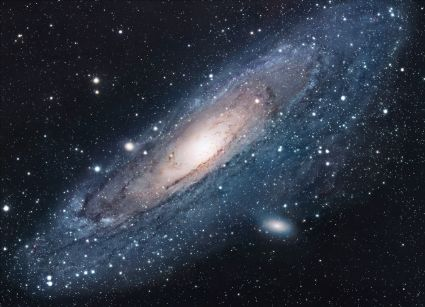
\includegraphics[scale=1.7]{universe.jpg}
\caption{The Universe}
\label{fig:univerise}
\end{figure}

\section{Conclusion}
``I always thought something was fundamentally wrong with the universe'' \citep{adams1995hitchhiker}

\bibliographystyle{plain}
\bibliography{references}
\end{document}
